% Inbuilt themes in beamer
\documentclass{beamer}

% Theme choice:
\usetheme{CambridgeUS}

% Title page details: 
\title{Assignment $4$\\ Probability and random Variables} 
\institute{Indian Institute of Technology Hyderabad}
\author{Shreyas Wankhede}
\date{\today}
\logo{\large \LaTeX{}}


\begin{document}

% Title page frame
\begin{frame}
    \titlepage 
\end{frame}

% Remove logo from the next slides
\logo{}


% Outline frame
\begin{frame}{Outline}
    \tableofcontents
\end{frame}


% Lists frame
\section{Question}
\begin{frame}{Question}

\textbf{CBSE class 12 Example 24}\\\vspace{5mm}
Two cards are drawn successively with replacement from a well shuffled deck of 52 cards.Find the probability distribution of the number of aces.\\

\end{frame}


% Blocks frame
\section{Solution}
\begin{frame}{Solution}
    The number of aces is a random variable.Let it be denoted by \textbf{X}. Clearly $\textbf{X} \in \{0,1,2\}$ \\
Now since the draws are done with replacement, the two draws form independent events.

\end{frame} 

\begin{frame}[t]{}
  \begin{align}
 \text{P} \{\textbf{X=0}\} &= \text{P}\{\text{non ace and non ace}\}\nonumber\\
 &=\dfrac{48}{52}\times\dfrac{48}{52}\nonumber\\
 &=\dfrac{144}{169}\label{eq:1}\\
  \text{P} \{\textbf{X=1}\} &= \text{P}\{\text{ace and non ace or non ace and ace}\}\nonumber\\
 &=\dfrac{4}{52}\times\dfrac{48}{52} + \dfrac{48}{52}\times\dfrac{4}{52}\nonumber\\
 &=\dfrac{24}{169}\label{eq:2}\\
  \text{P} \{\textbf{X=2}\} &= \text{P}\{\text{ace and ace}\}\nonumber\\
 &=\dfrac{4}{52}\times\dfrac{4}{52}\nonumber\\
 &=\dfrac{1}{169}\label{eq:3}
\end{align}  
\end{frame}

\begin{frame}{Table}
Thus from \eqref{eq:1}, \eqref{eq:2}, \eqref{eq:3} the required probability distribution is:\\
\begin{center}
\begin{tabular}{ |c|c|c|c| } 
 \hline
 \textbf{X} & $0$ & $1$ & $2$\\ 
 \hline
 \textbf{P}\{\textbf{X}\} & $\dfrac{144}{169}$ & $\dfrac{24}{169}$ & $\dfrac{1}{169}$  \\ 
 \hline
\end{tabular}
\end{center}
\end{frame}
    
\begin{frame}{plot (PMF)}
 \begin{figure}
 \vspace{-5mm}
 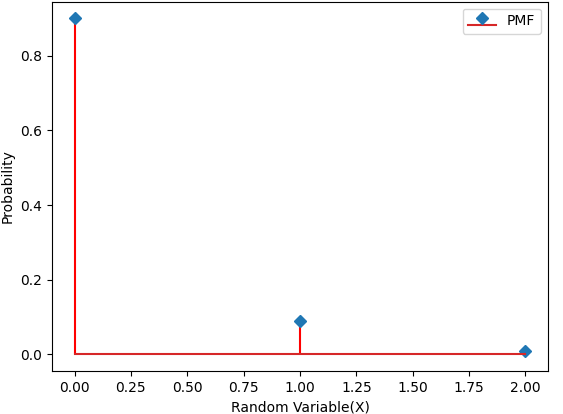
\includegraphics[width=3.4in,height=2.4in]{pmf_assgn_4.png}
\caption{PMF of distribution}
\label{fig-1}
\end{figure}   
\end{frame}

\begin{frame}{plot (CDF)}
 \begin{figure}
 \vspace{-5mm}
 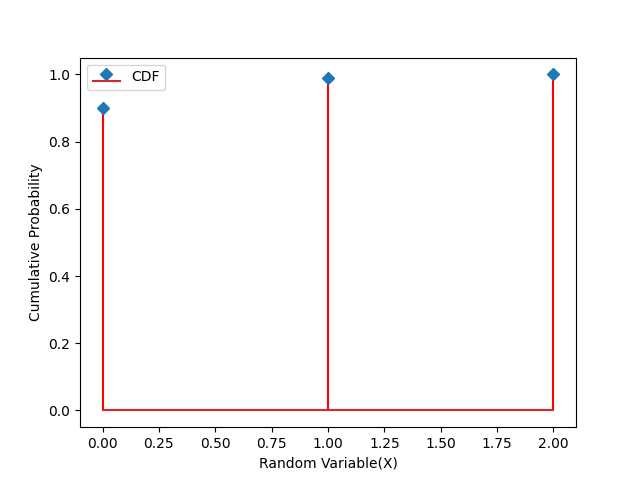
\includegraphics[width=3.4in,height=2.4in]{cdf_assgn_4.png}
\caption{CDF of distribution}
\label{fig-2}
\end{figure}   
\end{frame}



\end{document}